\documentclass[12pt]{article}
\usepackage{geometry}                		% See geometry.pdf to learn the layout options. There are lots.
\geometry{letterpaper}                   		% ... or a4paper or a5paper or ... 
%\geometry{landscape}                		% Activate for for rotated page geometry
%\usepackage[parfill]{parskip}    		% Activate to begin paragraphs with an empty line rather than an indent
\usepackage{graphicx}				% Use pdf, png, jpg, or eps� with pdflatex; use eps in DVI mode
								% TeX will automatically convert eps --> pdf in pdflatex		
\usepackage{amssymb}
\setlength{\parindent}{0pt}



\begin{document}

\begin{titlepage}

\newcommand{\HRule}{\rule{\linewidth}{0.5mm}} % Defines a new command for the horizontal lines, change thickness here

\center % Center everything on the page
 
%----------------------------------------------------------------------------------------
%	HEADING SECTIONS
%----------------------------------------------------------------------------------------

\textsc{\LARGE}\\[1.5cm] % Name of your university/college
\textsc{\Large Computer System Engineering}\\[0.5cm] % Major heading such as course name
\textsc{\large Design Project 1 Proposal}\\[0.5cm] % Minor heading such as course title

%----------------------------------------------------------------------------------------
%	TITLE SECTION
%----------------------------------------------------------------------------------------

\HRule \\[0.4cm]
{ \huge \bfseries Create a Versioning File System}\\[0.4cm] % Title of your document
\HRule \\[1.5cm]
 
%----------------------------------------------------------------------------------------
%	AUTHOR SECTION
%----------------------------------------------------------------------------------------

% If you don't want a supervisor, uncomment the two lines below and remove the section above
\Large \emph{Author:}\\
Bo Song  \textsc{11302010003}\\% Your name
YiTing Cheng  \textsc{11302010050}\\% Your name
YuWei Zhou  \textsc{11302010067}\\[3cm]% Your name

%----------------------------------------------------------------------------------------
%	DATE SECTION
%----------------------------------------------------------------------------------------

{\large \today}\\[3cm] % Date, change the \today to a set date if you want to be precise

%----------------------------------------------------------------------------------------
%	LOGO SECTION
%----------------------------------------------------------------------------------------

%\includegraphics{Logo}\\[1cm] % Include a department/university logo - this will require the graphicx package
 
%----------------------------------------------------------------------------------------

\vfill % Fill the rest of the page with whitespace

\end{titlepage}
\section*{Overview}
The goal of this design project is to create a versioning file system. The versioning or continuous snapshotting file system is defined to store all versions of each file over time. When users modifies a file(specifically, write or truncate something in a file) or modifies a directory(add, delete or rename files in it), the versioning file system create a new version after closing the file or directory and store the old version which can be only read by users. The system can be realized by extending inodes, interfaces and adopting copy-on-write memory management strategy based on Unix file system. 
\section*{Design Description}
\subsection*{Data Structure}To implement different versions of a file, some extra fields are added to the inode structure as follows(Figure 1).
\begin{description}
\item [Timestamp] - When a new version is created, a unsigned integer is recorded, representing the number of seconds passed since a epoch which is predefined in the system.
\item[Bitmap] - Maintaining the block versioning state of file or directory, in order to realize COW memory management, checking whether a new version is needed and performance optimization.
\item[Next] - A pointer to the next old version of an inode.
\item[Record] - A bit to indicate whether an user excludes the file or directory from versioning. Zero is default which is not excluded.
\item[Head Pointer] - A pointer to a block containing addresses of the head of sublists of inodes discussed in the layout section. 
\end{description}
\begin{figure}[!ht]
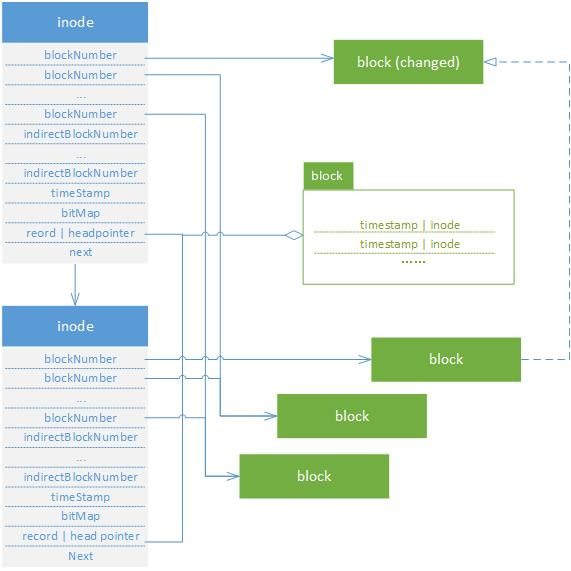
\includegraphics{figure1.jpg}
\caption{Data Structure and COW}Five new fields are added to inode. A head pointer points to a block containing the timestamp and address of each sublist head. The block pointers in inode only point to different blocks when the old block is updated.\\[0.5em] \hrule
\end{figure}
\subsection*{Memory Management}
When a new version is created, it is waste to copy all the block in the old version. So copy-on-write(COW) is adopted to implement multiple versions of data compactly. When we open a file, we duplicate the inode first. The duplicated inodes initially share all data blocks(including direct and indirect blocks) in common(Figure 1). When a block is update, which means writing or truncating in a file or add or delete files in a directory, the file system allocates a new physical block to hold the new data and change the block address and the related bitmap in the inode. When the user close the file, the new version of inode is finally created with only a few extra blocks. If there is no modification, which means bitmap is all zero, the duplicated inode will release. The COW strategy extremely improve the memory utilization in the system.
\subsection*{Layout}
The problem that the length of a linked inodes list may be very long will cost more time to find a specific old version. Hence, a optimized layout is introduced to solve this problem. When the length of linked list exceeds a predefined number, the system divides it into small sublists. The head of each sublist which contains the address of first inode in the sublist and its timestamp is recorded in a block mentioned in data structure section(Figure 2). When the user find a version of file with given timestamp, the system use the timestamp as a key and search the sublist containing that inode efficiently with a function. \\When the disk is almost full, the system also support garbage collection which frees the oldest sublist.\\[0.5em] 
\begin{figure}[!ht]
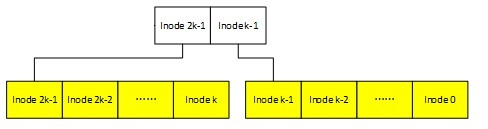
\includegraphics{figure3.png}
\caption{Layout}Constant k is predefined max length of sublist. White block is head block reference stored in head pointers block(Figure 1) and yellow block is linked sublist inode block.\\[0.5em] \hrule
\end{figure}
\subsection*{Manipulating Old Versions}
User can access any version of file or directories by appending @ and timestamp, such as ``cd $\backslash$home@1032433". When the system resolve the file or directory names, it reads from right to left and regard the last @ and number as version specifier. Hence, it can distinguish the version specifier from @ and numbers in its origin name.\\
Since the timestamp is not user-friendly, it has two extra ways to get the version we want.The first one is to lookup the log file or use list\_version system call to enumerate all the version of a file or directory. The other approach is use a inaccurate  timestamp and the layout in previous section will choose a sublists and result in a nearest version.
\section*{Conclusion}
The above design meets the requirements as outlined in the problem statement by strengthening inode structure. Although we employ copy-on-write strategy to reduce a lot of space cost, the system tends to sacrifice space for time such as bitmap  in each inode and extra blocks used in the file system layout. Future questions that still remain are the specifics of the implementation, as well as a better layout algorithm and use case analysis.\\[15em]

Word Count:797



\end{document}  